%%%%%%%%%%%%%%%%%%%%%%%%%%%%%%%%%%%%%%%%%
% University/School Laboratory Report
% LaTeX Template
% Version 3.1 (25/3/14)
%
% This template has been downloaded from:
% http://www.LaTeXTemplates.com
%
% Original author:
% Linux and Unix Users Group at Virginia Tech Wiki 
% (https://vtluug.org/wiki/Example_LaTeX_chem_lab_report)
%
% License:
% CC BY-NC-SA 3.0 (http://creativecommons.org/licenses/by-nc-sa/3.0/)
%
%%%%%%%%%%%%%%%%%%%%%%%%%%%%%%%%%%%%%%%%%

%----------------------------------------------------------------------------------------
%	PACKAGES AND DOCUMENT CONFIGURATIONS
%----------------------------------------------------------------------------------------

\documentclass{article}

\usepackage[a4paper, total={6in, 9in}]{geometry}

\usepackage{siunitx} % Provides the \SI{}{} and \si{} command for typesetting SI units
\usepackage{graphicx} % Required for the inclusion of images
\usepackage{amsmath} % Required for some math elements 
\usepackage[italian]{babel}
\usepackage{booktabs}% Better table spacing
\usepackage{subcaption}
\usepackage{tikz}

\setlength\parindent{0pt} % Removes all indentation from paragraphs

\renewcommand{\labelenumi}{\alph{enumi}.} % Make numbering in the enumerate environment by letter rather than number (e.g. section 6)

%\usepackage{times} % Uncomment to use the Times New Roman font

\usepackage{tikz}
\usetikzlibrary{positioning}
\tikzset{%
  every neuron/.style={
    circle,
    draw,
    minimum size=1cm
  },
  neuron missing/.style={
    draw=none, 
    scale=4,
    text height=0.333cm,
    execute at begin node=\color{black}$\vdots$
  },
}

%----------------------------------------------------------------------------------------
%	DOCUMENT INFORMATION
%----------------------------------------------------------------------------------------

\title{Ising and XY neural network} % Title

\author{Martina \textsc{Crippa}, Pietro Francesco \textsc{Fontana}} % Author name

\date{\today} % Date for the report

\begin{document}

\maketitle % Insert the title, author and date

%\begin{center}
%\begin{tabular}{l r}
%Date Performed: & January 1, 2012 \\ % Date the experiment was performed
%Partners: & James Smith \\ % Partner names
%& Mary Smith \\
%Instructor: & Professor Smith % Instructor/supervisor
%\end{tabular}
%\end{center}

% If you wish to include an abstract, uncomment the lines below
% \begin{abstract}
% Abstract text
% \end{abstract}

%----------------------------------------------------------------------------------------
%	SECTION 1
%----------------------------------------------------------------------------------------

\section{Introduzione}
Alcuni sistemi fisici presentano diverse fasi e al variare della temperatura transiscono da una fase all'altra. La temperatura a cui avviene questo passaggio di fase viene detta temperatura critica. In generale la transizione di fase è descritta da un parametro d'ordine, ad esempio la magnetizzazione nel modello di Ising. L'obiettivo del progetto è implementare e studiare una rete neuronale in grado di apprendere il parametro d'ordine e quindi classificare correttamente la fase di diverse configurazioni di un sistema, individuando infine la temperatura critica. Successivamente si è provato ad eseguire una procedura analoga nel caso di un sistema che non presenta una transizione di fase descrivibile attraverso un parametro d'ordine, quindi dove la rete neuronale apprende altre caratteristiche del sistema per classificarne la fase.
Il lavoro prende spunto da diversi articoli pubblicati negli ultimi due anni che affrontano la stessa tematica \cite{carrasqu,melko,wessel}.

%----------------------------------------------------------------------------------------
%	SECTION 2
%----------------------------------------------------------------------------------------

\section{Sistemi fisici e simulaizoni}
In questo lavoro sono stati simulati e studiati due sistemi matematici su reticolo bidimensionale:  il modello di Ising e il modello XY.
\subsection{Modello di Ising}
Il modello di Ising descrive il comportamento di spin su reticolo che possono assumere valori $+1$ o $-1$ ed interagiscono tra loro secondo un'hamiltoniana, la cui versione più semplice da trattare assume la forma
\begin{equation}
H(\sigma) =- \sum_{\langle i~j\rangle} \sigma_i\sigma_j
\end{equation} 
dove le parentesi angolari indicano l'interazione a primi vicini fra gli spin. L'energia di interazione è costante fra tutti gli spin e posta pari a $1$. Ad alte temperature il contributo entropico fa si che il sistema si trovi in uno stato di disordine, ovvero nella fase paramagnetica \ref{fig:isingP}. Abbassando la temperatura prevale il contributo energetico quindi al di sotto della temperatura critica gli spin tendono ad allinearsi e il sistema transisce alla fase ferromagnetica \ref{fig:isingF}.
\begin{figure}[h]
\centering
\begin{subfigure}[b]{0.4\linewidth}
\centering
\begin{tikzpicture}[> = stealth, scale=0.8]
\draw[gray,dashed,step=1.5cm] (-1,-1) grid +(5cm,5cm);
    \draw[ultra thick,red, <-]  (0,-0.50) -- (0,0.50);
    \draw[ultra thick,blue, ->]  (0,1) -- (0,2);
    \draw[ultra thick,blue, ->]  (0,2.5) -- (0,3.5);


    \draw[ultra thick,blue, ->]  (1.5,-0.50) -- (1.5,0.50);
    \draw[ultra thick,red, <-]  (1.5,1) -- (1.5,2);
    \draw[ultra thick,red, <-]  (1.5,2.5) -- (1.5,3.5);


    \draw[ultra thick,blue, ->]  (3,-0.50) -- (3,0.50);
    \draw[ultra thick,red, <-]  (3,1) -- (3,2);
    \draw[ultra thick,blue, ->]  (3,2.5) -- (3,3.5);
\end{tikzpicture}
\caption{Paramagnetico} \label{fig:isingP}  
\end{subfigure}
\begin{subfigure}[b]{0.4\linewidth}
\centering
\begin{tikzpicture}[> = stealth, scale=0.8]
\draw[gray,dashed,step=1.5cm] (-1,-1) grid +(5cm,5cm);
    \draw[ultra thick,blue, ->]  (0,-0.50) -- (0,0.50);
    \draw[ultra thick,blue, ->]  (0,1) -- (0,2);
    \draw[ultra thick,blue, ->]  (0,2.5) -- (0,3.5);


    \draw[ultra thick,blue, ->]  (1.5,-0.50) -- (1.5,0.50);
    \draw[ultra thick,blue, ->]  (1.5,1) -- (1.5,2);
    \draw[ultra thick,blue, ->]  (1.5,2.5) -- (1.5,3.5);


    \draw[ultra thick,blue, ->]  (3,-0.50) -- (3,0.50);
    \draw[ultra thick,blue, ->]  (3,1) -- (3,2);
    \draw[ultra thick,blue, ->]  (3,2.5) -- (3,3.5);
\end{tikzpicture}
\caption{Ferromagnetico} \label{fig:isingF}  
\end{subfigure}
\caption{Ising 2D}
\end{figure}  \\
Il parametro d'ordine che evidenzia la transizione di fase è la magnetizzazione totale del sistema:
\begin{equation}
M=\sum_i \sigma_i
\end{equation}
Sono stati studiati sistemi caratterizzati da tre distinte tipologie di reticolo, e conseguentemente aventi un numero di primi vicini (nn) e temperatura critica divera, i cui valori sono riportati in tabella \ref{tab:lt}:
\begin{table}[h]
\begin{center}
\begin{tabular}{lllll}
\toprule
reticolo & nn & $T_c$ & $T_c$ approx $[$\si{K}$]$ & $T_{init}$ $[$\si{K}$]$\\
\midrule
quadrato & $4$ & $2/ \!\ln{(1+\sqrt{2})}$ & $2.2692$ & $1.0$\\
triangolare & $6$ & $4/\!\ln{3}$ & $3.6410 $ & $2.0$\\
honeycomb & $3$ & $1/\!0.658478$ & $1.5187$ & $0.0$\\
\bottomrule
\end{tabular}
\end{center}
\caption{Reticoli studiati}
\label{tab:lt}
\end{table}\\
Per ciascuna tipologia di reticolo è stata variata la lunghezza del lato del reticolo (in numero di spin) da $20$ a $90$. La simulazione dei vari sistemi è stata effettuata con metodi Monte Carlo, equilibrando il sistema a temperatura fissata, in un range di $40$ temperature distribuite simmetricamente attorno alla temperatura critica, specificando la temperatura iniziale $T_{init}$ riportata in tabella \ref{tab:lt}.

\subsection{Modello XY}

%----------------------------------------------------------------------------------------
%	SECTION 3
%----------------------------------------------------------------------------------------

\section{Metodi di apprendimento}

A partire dai sistemi fisici simulati, descritti nella sezione precedente, sono stati sviluppati diversi metodi di apprendimento con l'obiettivo di classificare automaticamente la fase in cui si trova il sistema.
I metodi utilizzati per l'apprendimento differiscono per i due modelli fisici analizzati, il modello di Ising e il modello XY, seguendo la stessa strada di altri lavori.
%TODO citazioni!

\subsection{Modello di Ising}

\begin{figure}
\centering
\begin{tikzpicture}[x=1.5cm, y=1.5cm, >=stealth]

\foreach \m/\l [count=\y] in {1,2,3,missing,4}
  \node [every neuron/.try, neuron \m/.try] (input-\m) at (0,2.5-\y) {};

\foreach \m [count=\y] in {1,missing,2}
  \node [every neuron/.try, neuron \m/.try ] (hidden-\m) at (2,2.15-\y*1.35) {};

\foreach \m [count=\y] in {1,2}
  \node [every neuron/.try, neuron \m/.try ] (output-\m) at (4,1-\y) {};

\foreach \l [count=\i] in {1,2,3,n}
  \draw [<-] (input-\i) -- ++(-1,0)
    node [above, midway] {$I_\l$};

\foreach \l [count=\i] in {1,n}
  \node [above] at (hidden-\i.north) {$H_\l$};

\foreach \l [count=\i] in {1,2}
  \draw [->] (output-\i) -- ++(1,0)
    node [above, midway] {$O_\l$};

\foreach \i in {1,...,4}
  \foreach \j in {1,...,2}
    \draw [->] (input-\i) -- (hidden-\j);

\foreach \i in {1,...,2}
  \foreach \j in {1,...,2}
    \draw [->] (hidden-\i) -- (output-\j);

\foreach \l [count=\x from 0] in {di Input, nascosto, di Ouput}
  \node [align=center, above] at (\x*2,2) {Layer \\ \l};

\end{tikzpicture}
\caption{Schema di una rete neuronale \emph{feed forward} a singolo layer nascosto \emph{fully connected}.}
\label{fig:ffn}
\end{figure}

Per classificare le configurazioni di un modello di Ising è stata utilizzata una rete neuronale \emph{feed forward} a singolo layer nascosto, uno schema generico della rete è rappresentato in Figura \ref{fig:ffn}.
Al layer di input vengono fornite le configurazioni degli spin del sistema fisico nella forma di un vettore di elementi $\{+1;-1\}$, la dimensione di questo vettore dipende ovviamente dalla dimensione del reticolo di Ising utilizzato, nel caso del presente lavoro spazia da un minimo di 400 elementi (reticolo $20\times20$) ad un massimo di 8100 elementi (reticolo $90\times90$).
Si tratta di un problema di classificazione binaria, è quindi possibile utilizzare uno o due nodi nel layer di output, per una questione di comodità nell'analisi dei risultati fisici è stato utilizzato un layer di output a due nodi.
I nodi di output restituiscono la probabilità che la configurazione fisica sia in una fase ferromagnetica o in quella paramagnetica, le due probabilità sommano quindi a 1.

\subsection{Modello XY}

\begin{figure}
 \centerline{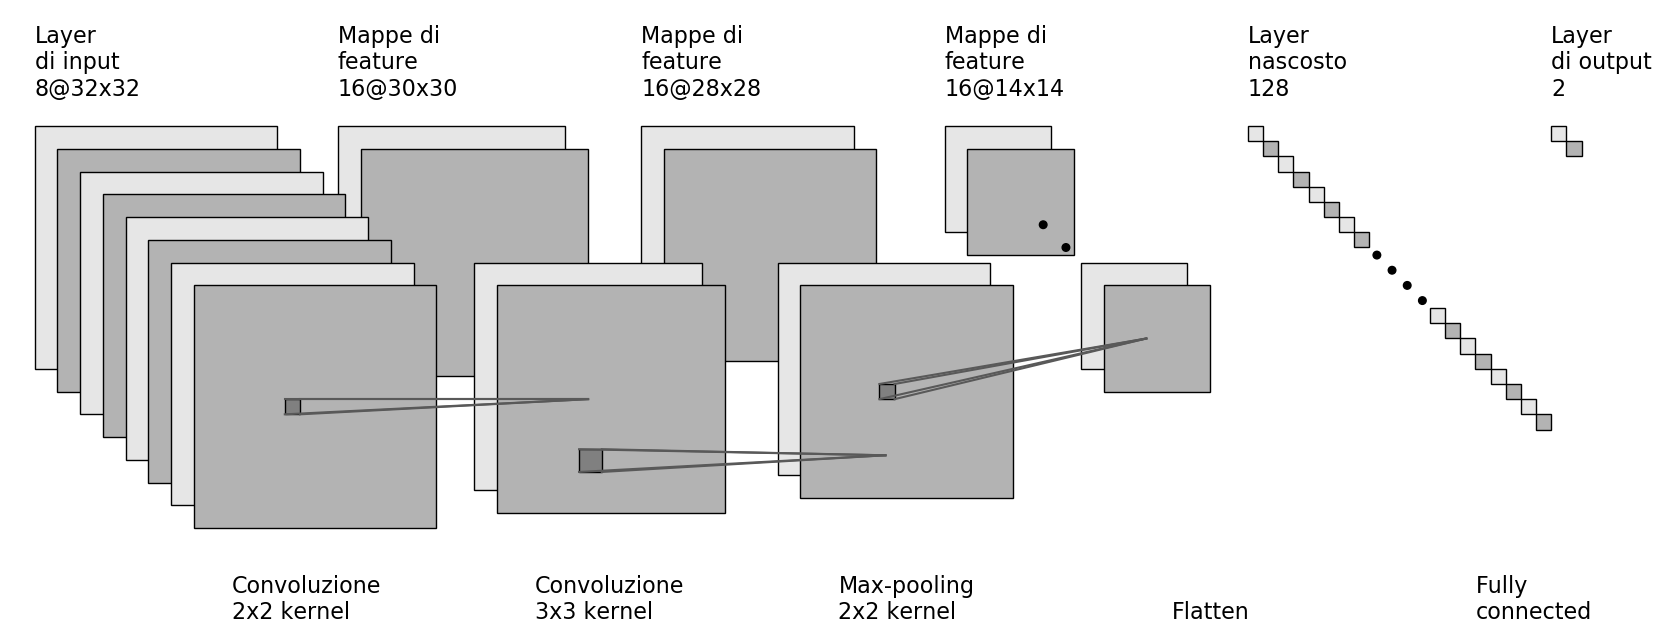
\includegraphics[scale=0.4]{cnn.png}}
 \label{fig:cnn}
 \caption{Schema di una rete convoluzionale effettivamente utilizzata per l'analisi di un sistema XY su reticolo $32\times32$, sono stati tralasciati i layer \emph{dropout}.}
\end{figure}


%----------------------------------------------------------------------------------------
%	SECTION 4
%----------------------------------------------------------------------------------------

\section{Risultati e conclusioni}

The atomic weight of magnesium is concluded to be \SI{24}{\gram\per\mol}, as determined by the stoichiometry of its chemical combination with oxygen. This result is in agreement with the accepted value.


%----------------------------------------------------------------------------------------
%	BIBLIOGRAPHY
%----------------------------------------------------------------------------------------

\bibliographystyle{ieeetr}

\bibliography{relazione}

%----------------------------------------------------------------------------------------


\end{document}
